\chapter{Documentation Technique}

    \section{Base de donnée}
        \subsection{Nettoyage du ficher source}
            Le fichier ressource qui nous avaient était fournis (\ilc{credit\_card\_fraud.csv}) avait eu besoin d'un petit nettoyage :
            \begin{diamond-enum}
                \item Les guillemets on étaient supprimées;
                \item Les virgules ont étaient replacés par des point, pour que les nombres soient proprement interprétés par la \ilc{DataFrame};
                \item Les point-virgules fûrent replacés simplement par des virgules.
                \item Les attributs de types numérique, ont étaient convertis en \ilc{float} ou en \ilc{int}.
                \item Les valeurs des champs \ilc{nameOrig} et \ilc{nameDest}, furent convertis en numérique avec le script :
                \begin{pybox}
                    def replace_first_letter(value):
                        if value.startswith('C'):
                            return '1' + value[1:]
                        elif value.startswith('M'):
                            return '2' + value[1:]
                        else:
                            return value
                \end{pybox}
            \end{diamond-enum}

        \subsection{MCD}
        La construction de la base de données a commencé par la réalisation du MCD, et par le passage au MPD avec le logiciel \emph{Looping}.
        Une fois celui-ci terminé, nous avons utilisé le module \ilc{mysql.connector} pour établir une connexion, et pour la construction de notre base de données depuis Python.
        \begin{figure}[ht]
            \centering
            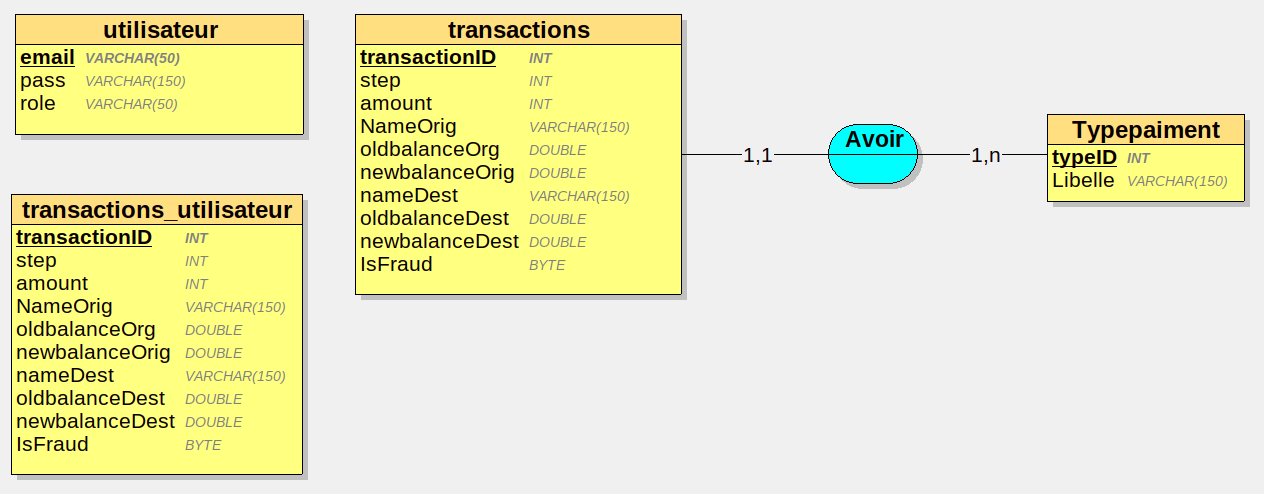
\includegraphics[width=0.8\linewidth]{\pres/db_mcd.png} % Replace "example-image" with your actual image file name
            \caption{MCD à partir du fichier \ilc{credit\_card\_fraud.csv}}
        \end{figure}